\documentclass[./A14_Report.tex]{subfiles}

\begin{document}
\chapter{Introduction}
\section{Overview}
The project aims to implement the \textbf{Embedded Zerotree Wavelet} algorithm
as a C library. It employs the well known \textit{Discrete Wavelet Transform}
as a tool for compression. The algorithm will be studied under several
operating conditions and demands, such as varying levels of
compression,``bit-budget'', etc

\section{The transform coder}

\begin{figure}[h]
    \centering
    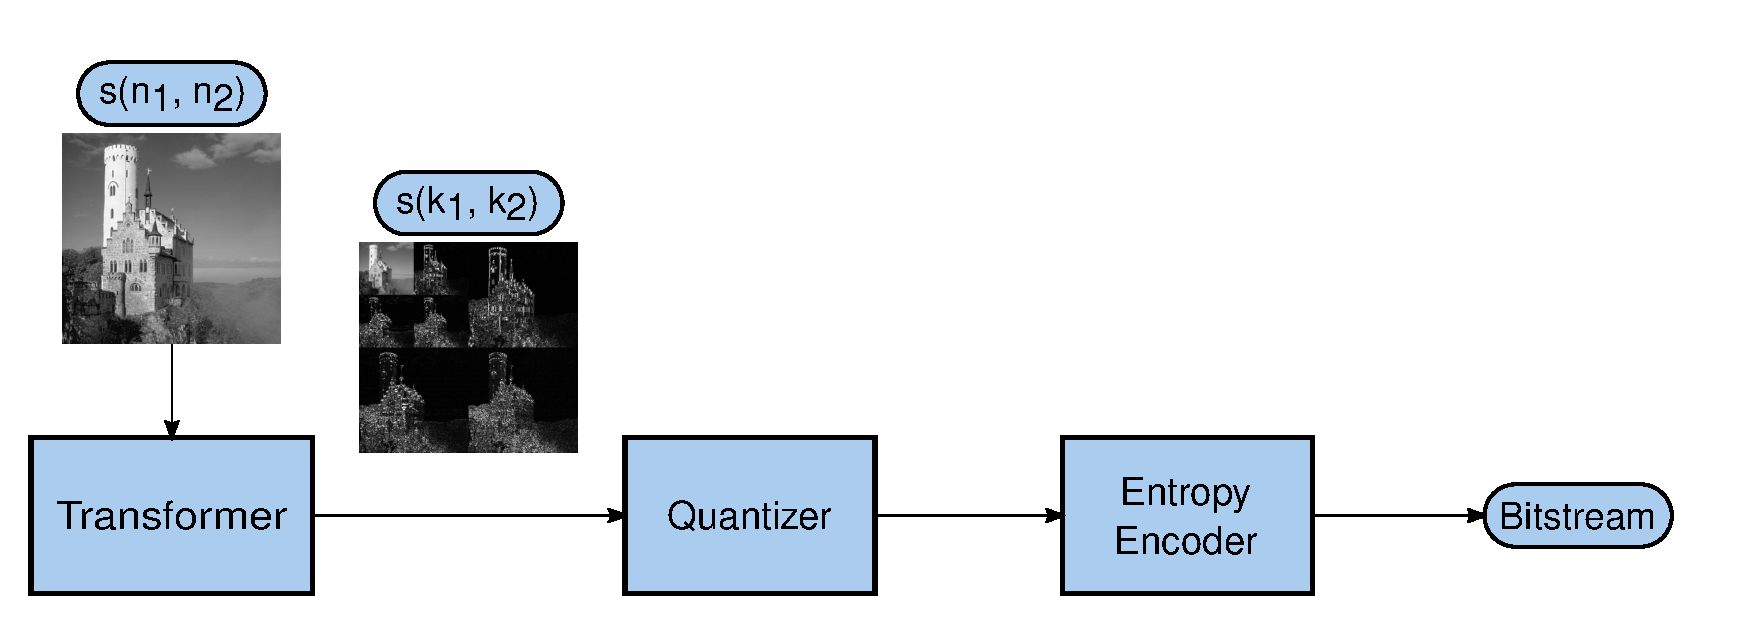
\includegraphics[scale=0.5]{../img/block-diag_shrunk.pdf}
    \caption{Transform coder: Generalised \cite{shap1993}}
    \label{fig:tcoder}
\end{figure}

A step-wise approach towards implementing this algorithm is taken, wherein
the each step is represented by a block in figure \ref{fig:tcoder}.

\pagebreak

\subsection{The transformer}
The transformer performs a mathematical transform on the supplied image. The
transform must satisfy 2 key properties, namely:
\begin{itemize}
    \item Full invertibility
    \item Separability
\end{itemize}

A few transforms that satisfy these conditions are the Fourier transform, the
discrete cosine transform and the wavelet transform. We will be using the
wavelet transform, since it is very handy when it comes to multi-resolution
analysis.

\subsection{The quantizer}

\subsection{The entropy encoder}
\end{document}

